\begin{sidewaysfigure}
	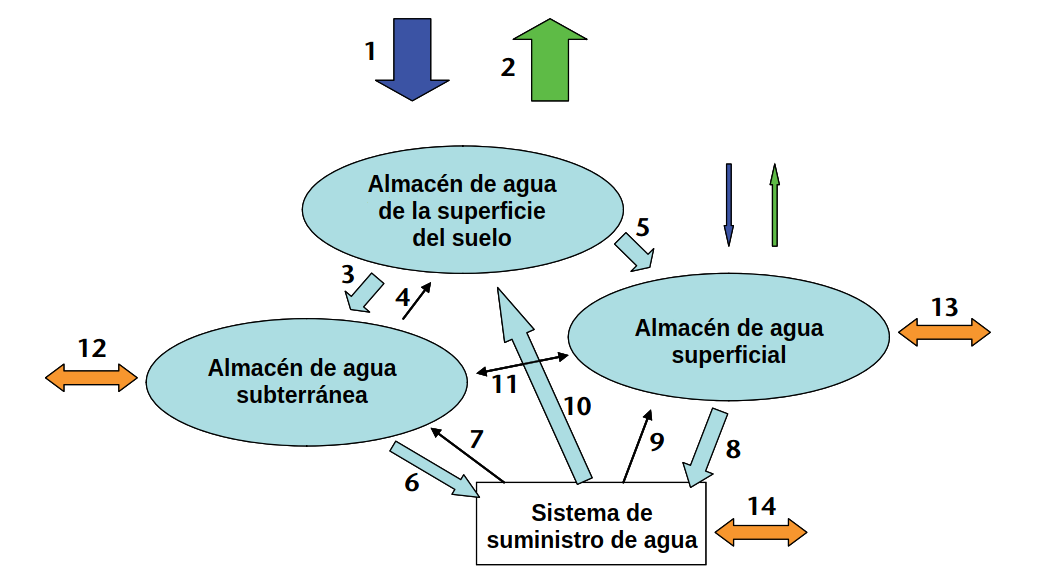
\includegraphics[scale=0.58]{Images/water_balance_wmo.png}
	\centering
	\caption{Diagrama conceptual del marco de balance hídrico en una cuenca. Los flujos (principales) enumerados son: 1) precipitación; 2) evapotranspiración; 3) recarga de agua subterránea; 4) ascenso capilar; 5) escorrentía, aguas pluviales; 6) extracción de agua subterránea; 7) fuga, inyección de acuífero; 8) desvío de aguas superficiales; 9) flujos de retorno (contaminados); 10) riego; 11) interacción de aguas subterráneas/superficiales; 12) flujo de agua subterránea dentro/fuera de la cuenca; 13) flujo de agua superficial dentro/fuera de la cuenca; y, 14) aguas residuales, flujo entre cuencas.}
	Fuente: \citet{WMO2012}.
	\label{fig:water_balance_wmo}
\end{sidewaysfigure}
